\documentclass[a4paper]{article}

%% Language and font encodings
\usepackage[english]{babel}
\usepackage[utf8x]{inputenc}
\usepackage[T1]{fontenc}

%% Sets page size and margins
\usepackage[a4paper,top=3cm,bottom=2cm,left=3cm,right=3cm,marginparwidth=1.75cm]{geometry}

%% Useful packages
\usepackage{amsmath}
\usepackage{graphicx}
\usepackage[colorinlistoftodos]{todonotes}
\usepackage[colorlinks=true, allcolors=blue]{hyperref}
\usepackage{subfigure}
\usepackage{caption}
\usepackage{amsfonts}
\usepackage{amsthm}
\usepackage{upquote}
\usepackage{listings}
\usepackage{enumitem}
\usepackage{dirtytalk}
\usepackage{hyperref}
\usepackage{float}

\usepackage{xcolor}
\usepackage{indentfirst}

\definecolor{mGreen}{rgb}{0,0.6,0}
\definecolor{mGray}{rgb}{0.5,0.5,0.5}
\definecolor{mPurple}{rgb}{0.58,0,0.82}
\definecolor{backgroundColour}{rgb}{0.95,0.95,0.92}
\lstdefinestyle{CStyle}{
    backgroundcolor=\color{backgroundColour},
    commentstyle=\color{mGreen},
    keywordstyle=\color{magenta},
    numberstyle=\tiny\color{mGray},
    stringstyle=\color{mPurple},
    basicstyle=\footnotesize,
    breakatwhitespace=false,
    breaklines=true,
    captionpos=b,
    keepspaces=true,
    numbers=left,
    numbersep=5pt,
    showspaces=false,
    showstringspaces=false,
    showtabs=false,
    tabsize=2,
    language=C
}


\def\therefore{\boldsymbol{\text{ }
\leavevmode
\lower0.4ex\hbox{$\cdot$}
\kern-.5em\raise0.7ex\hbox{$\cdot$}
\kern-0.55em\lower0.4ex\hbox{$\cdot$}
\thinspace\text{ }}}

\title{A Journey to the Interactive 3D Fractal World}
\author{CSED Yang Junha 20160785, Ryu Sangwoo 20160845, Sung Haebin 20160463}

\begin{document}
\maketitle
\begin{abstract}

\end{abstract}
\section{Motivation}

\section{Theoretical Backgrounds}
\subsection{Fractal}
\subsection{Mandelbrot Set}

\section{Task}
\subsection{Overall Structure}
\subsection{Tasks}


\section{Ideas and Implmentation}
\subsection{Development Enviornment}
\subsection{Rendering a Mandelbrot set}

\begin{lstlisting}[style=CStyle]
int main(void)
{
  printf("If you want to paste code here then do this way");
}
\end{lstlisting}
\subsection{3D Geometric Fractals}

\subsection{Texture Mapping}

\subsection{Deformations}

\subsection{Camera control}
\subsection{Antialiasing}


\section{Gallery}
\begin{figure}[H]
\centering
\subfigure[scene from a Youtube video(\url{https://youtu.be/S530Vwa33G0})]
{
    \label{fig:subfig1}
    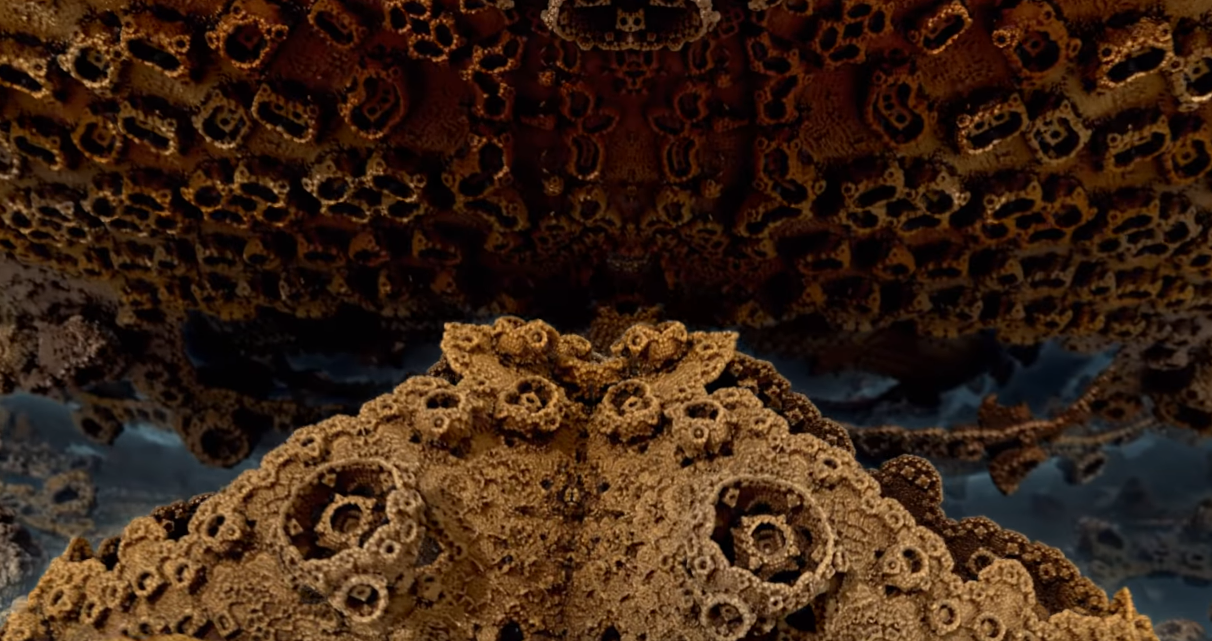
\includegraphics[scale=0.3]{cap1.PNG}
}
\end{figure}
\section{Discussion}
There are some issues in this project.
\begin{description}[style=nextline]
\item[hihi?]
byebye
\end{description}

\begin{thebibliography}{1}
\bibitem{c1}E. Angel and D. Shreiner, Interactive Computer Graphics: A Top-Down Approach with Shader-Based OpenGL, 6th ed., Addison-Wesley, 2011, p.487 Section 9.8 Recursive Methods and fractals
\bibitem{c2}Graham Sellers; Richard S. Wright, Jr.; Nicholas Hanemel, OpenGL SuperBible, 7th ed., Addison-Wesley, p.683 Rendering Julia Fractals
\bibitem{c3}Rickard Englund, Rendering Methods for 3D Fractals
\bibitem{c4}Fragmentarium,\url{http://syntopia.github.io/Fragmentarium/index.html}
\end{thebibliography}

\end{document}
